\section{Architectural Overview: Basic TC System}

The blockchain interface to \tc is the smart contract \tcont. \tcont is designed to present a simple API to a relying contract / requester \reqcont. \reqcont sends to \tcont a specification of the datagram it is requesting, along with payment. The datagram specification includes the data being sought and may also include parameters, such as the time at which the data should be retrieved, the target source or sources, and so forth. \tcont simply returns the requested data to \reqcont. The interaction between \reqcont and \tcont takes place entirely on the blockchain.

The complexity of \tc resides primarily in its backend, which must monitor, keep track of, and fulfill datagram requests passing from requesters through \tcont. Additionally, to validate the trustworthiness of \tc, the entity or entities creating \reqcont must verify a hardware- (SGX-)generated attestation. So \tc must also support a service to fulfill attestation requests off-chain. 

\subsection{Architecture}

The \tcs system includes three main components: The \tcontract, the \encname, and the \medname. The \encname and \medname reside on the \tc server, while the \tcontract resides on the blockchain. An architectural schematic showing the roles of these components is given in Figure~\ref{fig:overview}.

\vspace{-2mm}
\begin{figure}[h!]
\centering
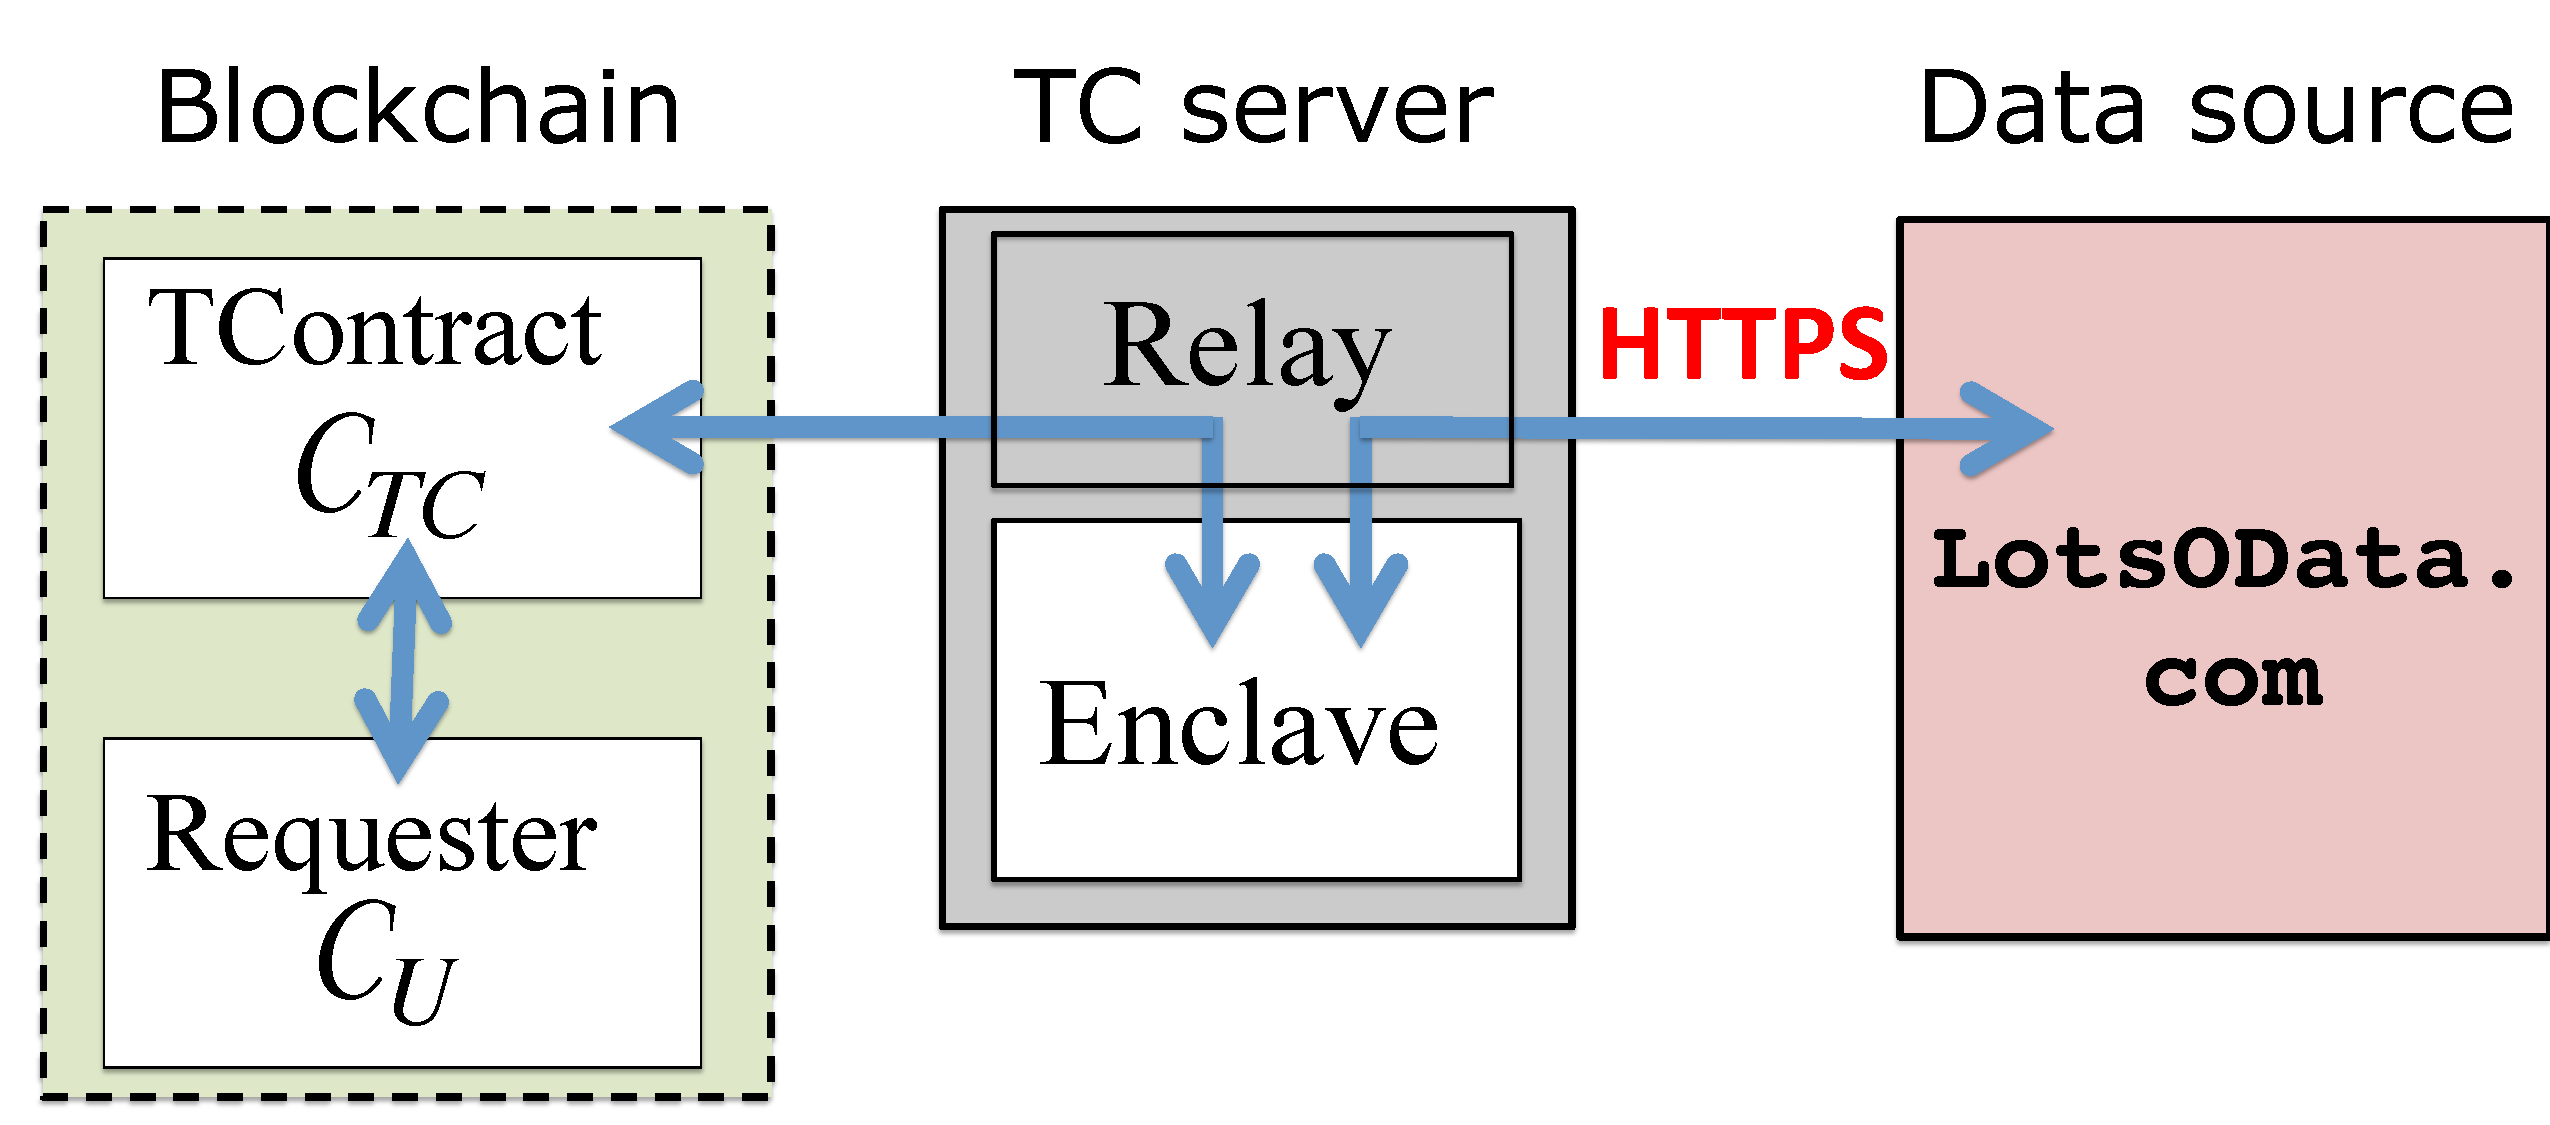
\includegraphics[width=\columnwidth]{figures/OverviewFig}
\caption{{\bf Basic Town Crier architecture.}}
\label{fig:overview}
\end{figure}
\vspace{-2mm}

\paragraph{The \tcontract (\tcont).} The \tcontract (denoted by \tcont) is a smart contract that acts as the blockchain front-end of the \tc service, and thus an interface between relying contracts and \tc. It accepts datagram requests from a requester \reqcont and returns corresponding datagrams from \tc. Additionally, the \tcontract manages \tc monetary resources, which in Ethereum take the form of ether (money) and gas (``fuel'' for contracts). 

\paragraph{The \encname.}
The \encname ingests and fulfills datagram requests from the blockchain. To obtain the data for inclusion in datagrams, it queries external data sources, specifically HTTPS-enabled internet services. It returns a datagram to a requesting contract \reqcont as a digitally signed blockchain message. The \encname runs in an SGX enclave, and is thus secured against an adversarial OS as well as other process on the host. 

\paragraph{The \medname.} As an enclave process, the \encname lacks direct network access. Thus the \medname handles bidirectional network traffic on behalf of the \encname. Specifically, the \medname provides network connectivity from the \encname to three different types of entities: 

\begin{enumerate}
\item {\em The Blockchain (the Ethereum system):}  The \medname scrapes the blockchain in order to monitor the state of the \tcontract  \tcont. In this way, it performs implicit message passing from \tcont to the \encname, as neither component itself has network connectivity. Additionally, the \medname places messages emitted from the \encname (datagrams) on the blockchain.
\item {\em Clients:} The \medname runs a web server to handle off-chain service requests from clients, specifically, requests for attestations from the \encname. As we soon explain, an attestation provides a unique public key for the \encname instance to the  client and proves that the \encname is executing correct code in an enclave and that its clock is correct in terms of absolute (wall-clock time). A client that successfully verifies an attestation can then safely create a relying contract \reqcont that uses the \tc.
\item {\em Data sources:} The \medname relays traffic to and from data sources (HTTPS-enabled servers) queried by \encname. 
\end{enumerate}

The \medname is an ordinary user-space application. It does not benefit from integrity protection by trusted hardware and thus, unlike the \encname, can be subverted by an adversarial OS on the \tc server, causing network delays or failures. As we explain in detail later in the paper, however, a key design aim of \tc is that \medname should be unable to cause incorrect datagrams to be produced or users to lose money. In general, the \medname~{\em can only mount denial-of-service attacks against \tc}. 

\paragraph{End-to-end datagram processing.}
In summary, then, a datagram request is initiated by a requester \reqcont. \reqcont sends a datagram request to \tcont on the blockchain. Using network services provided by the \medname, the \encname obtains the request from the blockchain. It contacts a data source to obtain the requested data and composes a datagram, which it sends back to \reqcont.

As a simple example, \reqcont might request a stock ticker  (e.g., the price of IBM at 3 p.m. on 15 Jan 2017). The \encname would fetch the requested data from an online service (e.g., https://www.google.com/finance) and place it in a datagram for transmission via \tcont to \reqcont.

%In addition to servicing datagram requests, the \encname may be queried by a client to provide an off-chain, hardware-backed attestation $\att$ on the state of the \encname---both its executing code and its clock. It is to support this service that \medname includes a web server. We do not depict this service in Figure~\ref{fig:overview}, and defer its discussion to later in the paper.

We now make this data flow more precise. 

\subsection{Datagram processing: Data flow}

We denote a datagram instance, namely the set of message values associated with a datagram request, by $\dgi$, where $i$ is a unique instance index. (We explain in Section~\ref{sec:implementation} how this index is computed.) 

A datagram request by \reqcont takes the form of a message $\dgi.\dgreq$ to \tcont on the blockchain. This message $\dgi.\dgreq = (\dgi.\dgform, \dgi.\dgpay)$ includes both a specification $\dgi.\dgform$ of the requested datagram (e.g., a stock ticker and desired time) and a payment $\dgi.\dgpay$, which in Ethereum may include gas to cover the execution cost of the request as well as a service fee. \tcont receives a return message $\dgi.\dgret = (\dgi.\dgform, \dgi.\dgm)$ from the $\tc$ service where $\dgm$ contains the data (e.g., the desired stock ticker price). \tcont checks the consistency of $\dgi.\dgform$ on the incoming and outgoing messages, and if they match forwards $\dgi.\dgm$ to \reqcont. Where clear from context, we omit the prefix $\dgi$ from our notation.

Figure~\ref{fig:dataflow} shows the data flows involved in processing a datagram request. For simplicity, the figure omits the \medname, which is only responsible for data passing.


\begin{figure}[h!]
\centering
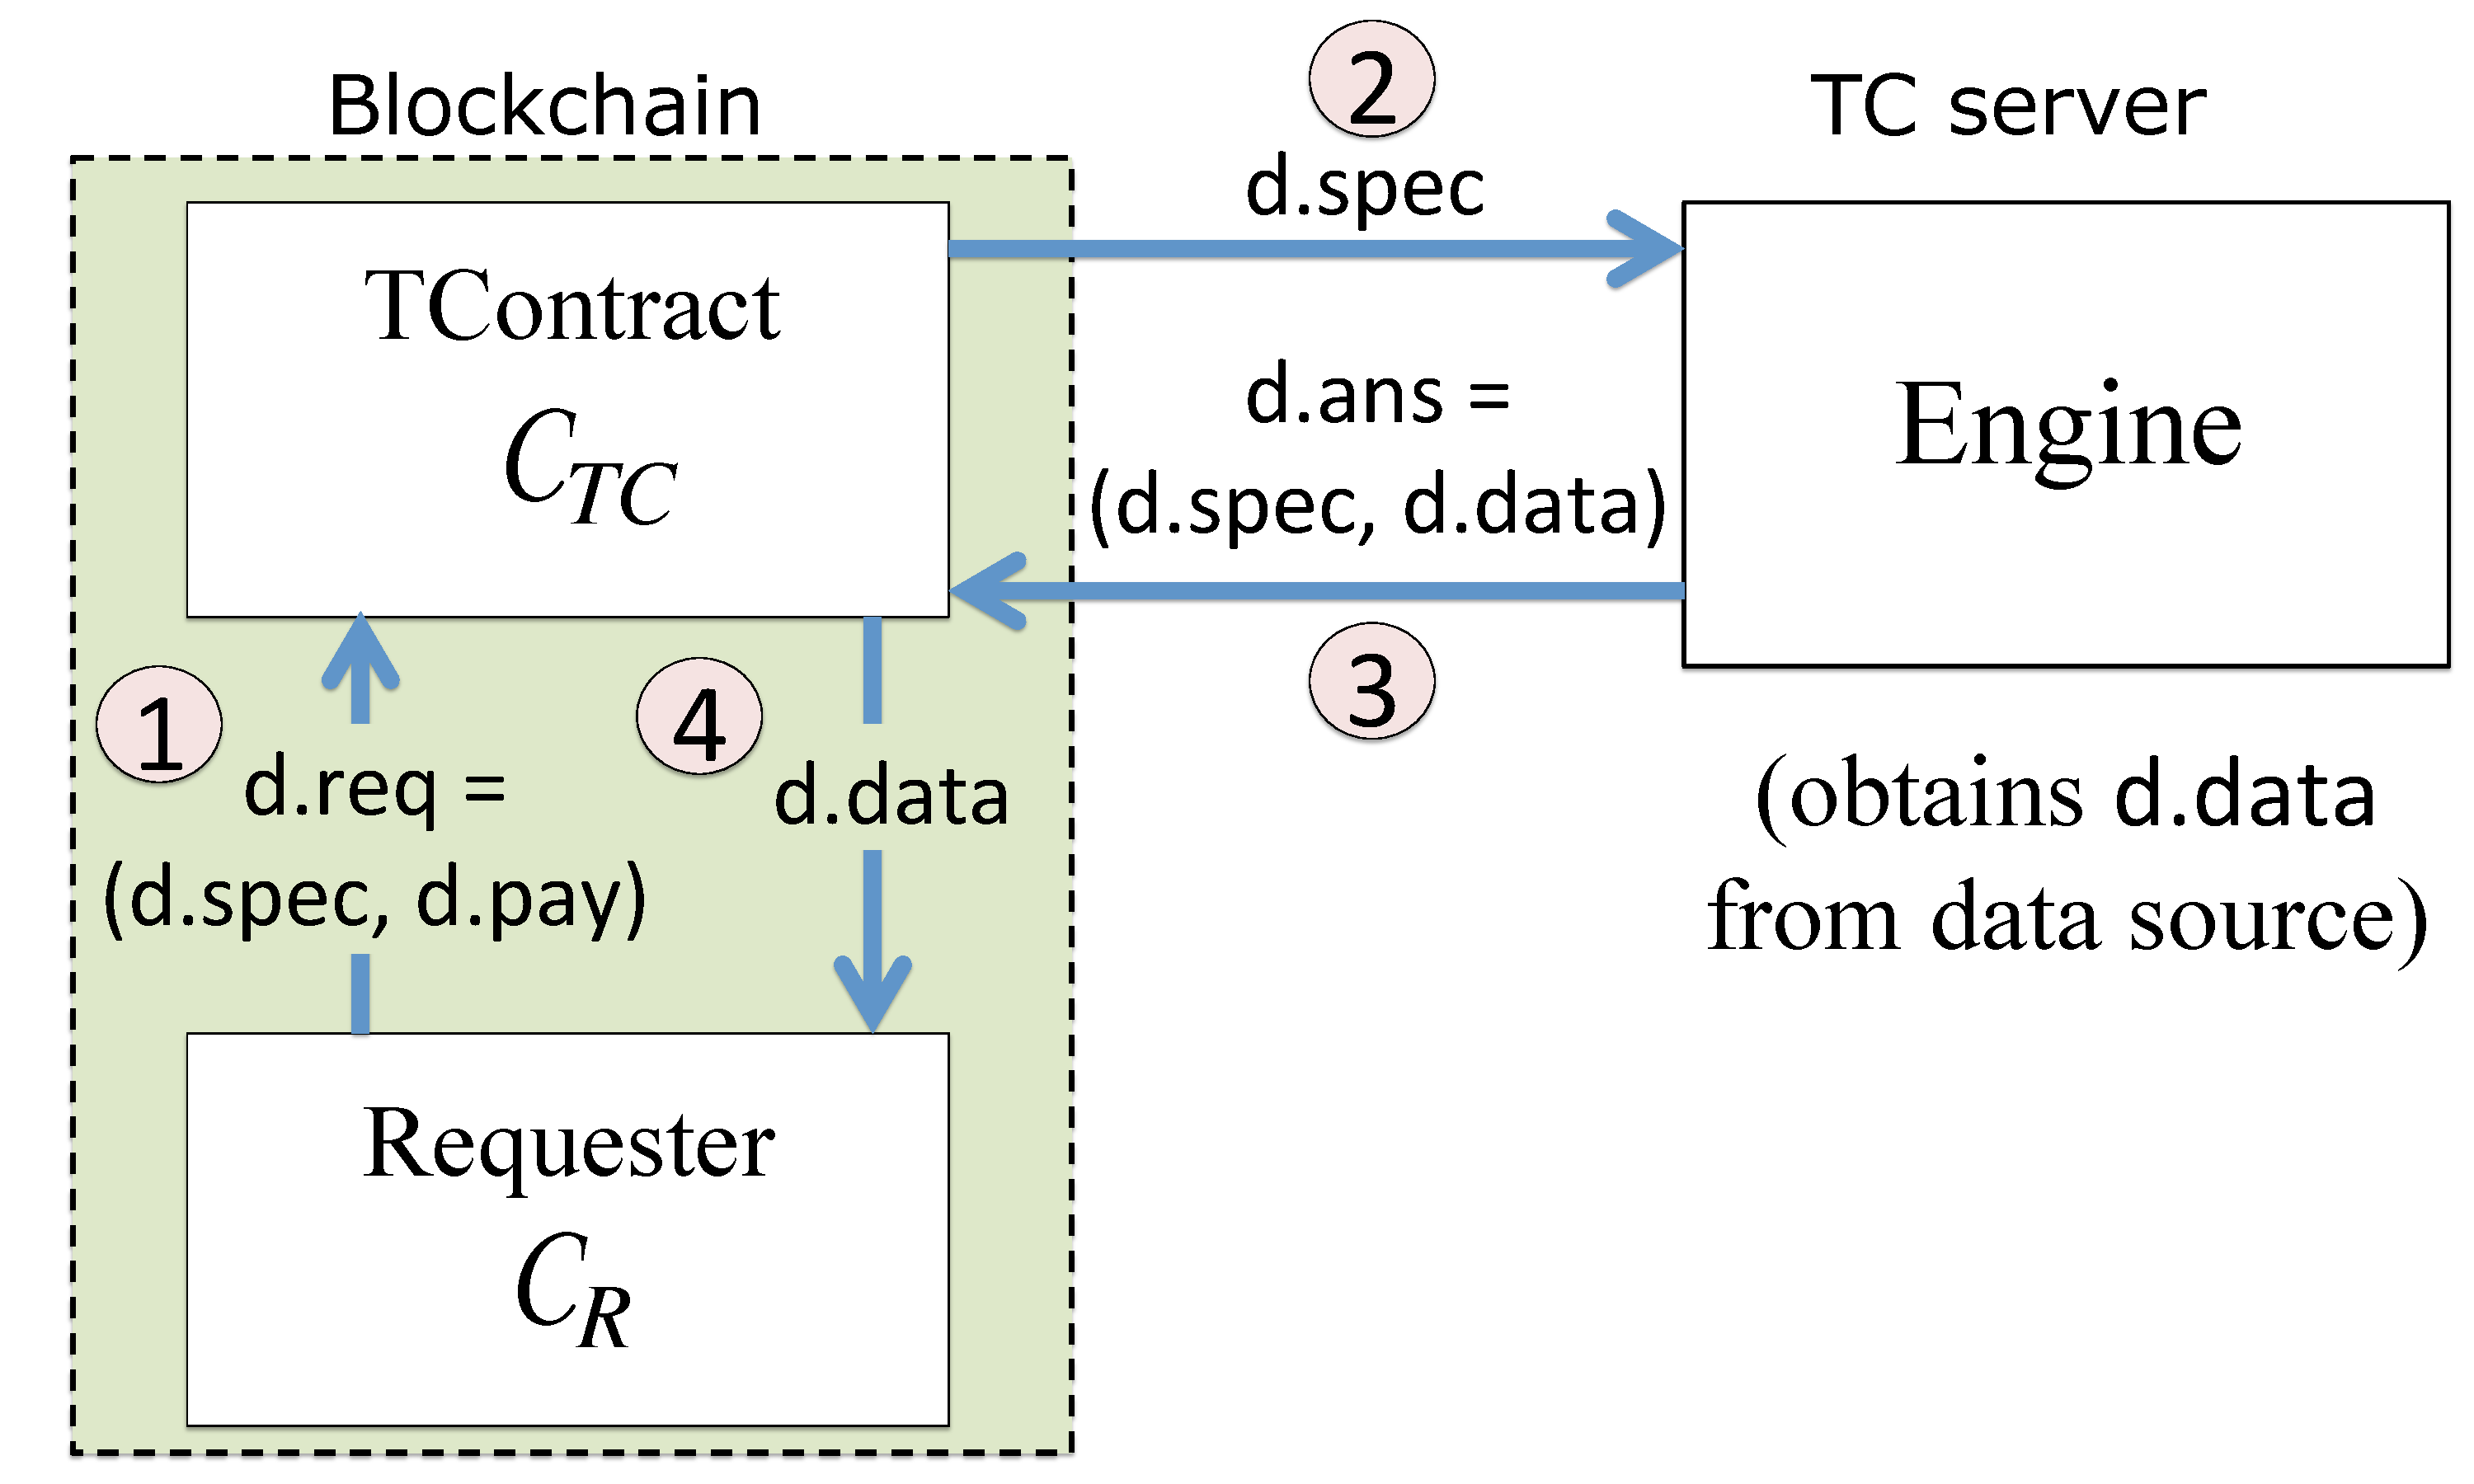
\includegraphics[width=\columnwidth]{figures/DataflowFig}
\caption{{\bf Data flows in datagram processing.}}
\label{fig:dataflow}
\end{figure}


Digital signatures are needed to authenticated messages, such as $\dgret$, entering the blockchain from an external source. We let $(\skTC, \pkTC)$ denote the private / public keypair associated with the \encname for such message authentication. For simplicity, we assume for the time that the \encname can send signed messages directly to \tcont. Later we explain how Ethereum requires a slightly different approach.

\subsection{Security model}

Here we given an overview of our security model for \tc, providing more details in our security analysis in section~\ref{}. We assume the following:

\begin{itemize}
\item {\em \encname security:} Leveraging the basic properties of SGX, an attestation $\att$ proves to a verifier (client) about an \encname instance that: (1) The instance is executing correct code, i.e., behaves honestly; (2) For a public key $\pkTC$ included in the attestation, the corresponding private key $\skTC$ is known only to the instance; and (3) The SGX / enclave clock is set to absolute (wall-clock) time $T$ asserted in $\att$, where $T$ is verifiable by a client (requesting a fresh attestation) to within accuracy $\Delta$ (e.g., 100ms).

\item {\em Network communication:} The \medname (and other untrusted components of the \tc server) can tamper with or delay communications to and from the \encname, but cannot otherwise observe or alter the behavior of the \encname. Thus the \medname is simply subsumed by an adversary that controls the network. 

\item {\em Blockchain communication:} Message sources are authenticable, i.e., the originating blockchain address of a message can be correctly identified, and messages are integrity protected, but not confidential. This includes messages sent from the \encname, whose public key $\pkTC$ is bound in \tc to a blockchain account. 
\end{itemize}

\subsection{Design rationale: Role of \tcont}

One could imagine an alternative strawman protocol such as the following...

It is perhaps not immediately evident why our architecture makes use of the contract \tcont to intermediate between \reqcont and the \encname. In principle the \tc service could scrape the blockchain, identify contracts with state explicitly indicating a request for datagrams and send them datagrams and accompanying attestations directly.  This would result in a conceptually simpler protocol, eliminate some in-blockchain message passing, and also ensure that \reqcont consumes only fresh SGX attestations. In contrast, in our design, it is most practical for users to verify an SGX attestation offline at the time \reqcont is created, raising the risk that the attestation goes stale. (Of course, revocation must be handled in either case.)

The rationale for this design choice is twofold: First, \tcont manages the payment of fees (ether and gas) for the \tc service, creating a fair exchange of datagrams for fees. Second, although \reqcont could in principle verify a TC attestation directly, in practice, this would not be practical today. In Ethereum, opcodes for in-contract cryptographic operations are very limited and do not currently support public-key cryptography. (Digital signatures are supported only for messages from non-contract accounts.) 










